\documentclass[11pt]{article}
\usepackage[utf8]{inputenc}
\usepackage{hyperref}
\usepackage{amsmath}
% \usepackage{geometry}
\usepackage{amsmath}
\usepackage{graphicx}
\usepackage{epigraph}
\usepackage{biblatex}
\usepackage{url}
%\usepackage{subfigure}
\addbibresource{references.bib}
% \setlength{\parskip}{1em}
\usepackage{float}
\usepackage{subfig}
\usepackage{soul}
\usepackage{tabularx}
% \geometry{margin=1in}

\title{Mozart Simulator}
\author{Paul Smith, Luke Wright, Bryce Lunceford, Daniel Smith, Erika Ibarra}

\begin{document}
\maketitle
\begin{abstract}
Automatic music generation is a relatively new frontier in the world of data science. In the following project, this medium was explored on the specific style of Mozart sonatas. While there could be many approaches for generating music, this project attempted to employ \textit{Hidden Markov Models} (HMMs) and \textit{Random Forests} to generate unique and original compositions worthy of Mozart's repertoire. The resulting music, though promising, demonstrates the difficulty of non-neural approaches in music generation.
\end{abstract}

\section{Problem Statement}
Computer generated music was first seen in the late 1950s with the creation of, The Silver Scale, a melody produced at Bell Laboratories. The duration of this simple composition was 17 seconds \cite{Briot}. It was a breakthrough 
accomplishment, even if it did sound like a strange sci-fi jingle. With many notable advancements in the domain of machine learning, algorithm generated music has since become much more sophisticated. Today, one can easily peruse the internet and find modules like Musenet \cite{payne_2021}, developed from the research 
of OpenAI, which can analyze anything from Beethoven to the Beatles, calculate the style, and synthesize a similar or complementary composition that utilizes sounds from a handful of different instruments. The techniques most commonly used to support computer generated music come from Deep Learning and Deep Neural Networks. However, research suggests that simpler Markov models can be used as well. With that being said, there are trade-offs.

Markov models are relatively simple to use, they can learn from a small set of data, and they can often be implemented with a control. However, they may not be as good at capturing long term structures or generalizing as well as their Neural Network counterparts. The objective of this project is to test the hypothesis that Markov models can be used to accurately synthesize music.

Altogether, the motivation for this project comes down to supporting art. Music is a huge part of human culture. It can influence feelings, encourage behaviors, and ultimately shape who we are. But music is also expensive to produce. Creating an algorithm that is capable of replicating the general style of Mozart piano sonatas could not only help individuals inherit the benefits of listening to his music, but it could
provide such benefits cheaply, and in the form of new music each and every time. 

\section{Data}
The data we used was a series of midi files with recordings of
Mozart piano sonatas. These recordings were accurate renditions of
Mozart's music, so we didn't have to worry about any missing data or
inaccuracies. Midi files are also constructed in a convenient manner that
breaks the recording into individual timesteps and describes what happens to 
each note at each timestep. Using this information, we created an $n \times 88 
\times 2$ array (where $n$ is the number of timesteps in the piece). For 
each timestep, the first column describes which of the $88$ possible notes 
are being played (there are 88 notes on a piano keyboard), 
and the second column describes the speed at which the 
corresponding notes are being played; this speed refers to the speed at which
the action of the key is pressed, not how long the note is played for.
This array we created (hereafter called the Master Array), provided a simple
way for us to work with out data. To train on multiple pieces of music, we
simply concatenated the pieces' Master Arrays into a single array.
    
\section{Methods}
\subsection{State Space Dimension Reduction}
Each note of the Master Array can take on three values for a given timestep:
 $1$ signifies that the note is being pressed, $-1$ signifies that the 
note is being depressed, and $0$ signifies that the state of the note has 
not changed. Since there are $88$ possible notes that could be played at any
given timestep, and each note could take on $3$ different values, each
timestep has $3^{88}$ possible values. To decrease the dimension size of
our data, we assigned a single integer to each unique combination of
notes played throughout the piece. This decreased the dimension size of our
data from $3^{88}$ to only a few hundred. We then assigned each of these numbers
to their corresponding timestep so that we had a single array of integers with
length $n$. We used the same technique to also lower the dimension size of
the note speeds.

\subsection{Cleaning Generated Music}
We found that generated music often contradicted physical possibility. Specifically, there were two problem cases we needed to address whenever we generated new music: $(1)$ a note could be depressed before it was pressed, and $(2)$ a note could be pressed twice without ever being depressed.
In both cases, we decided to ignore the problematic action and set the note value to $0$. Admittedly, there wasn't much precedent for this decision, but it seemed better than directly altering the composition by pressing or depressing the note.

In addition to cleaning the note values, the speed values also needed to be cleaned. One issue that arose when attempting to assign speed values to notes was that the number of notes and the number of speeds that were generated for a particular timestep were not always the same. To solve this problem, if the number of nonzero speeds in the speeds array
was not equal to the number of notes being pressed in a given timestep, we
simply assigned the mean of the speeds to each note not already assigned a speed. After this cleaning, we had a new Master Array where each note was pressed and
depressed with an associated speed as expected. We then used this new
Master Array to construct a midi file which could be played to hear the song.

\subsection{Attempt 1: Hidden Markov Model}
We used an \textit{HMM} to create a model that tried to accurately simulate how
the inputted music is constructed using a given number of hidden states 
(which we initially tested with $20$ states). We fit the model using the Baum-Welch algorithm, and we sampled from the resulting model to generate a new sequence of notes to be played. However, to determine the speeds of each note, 
we had to use a different approach. Using the Viterbi algorithm, we assigned each note from the original composition to a hidden state. Then, we found a distribution over the speed values by counting the frequency of each speed associated with each hidden state. To assign a speed value to each new note, we looked at the hidden state it belonged to, and then drew a random sample from the speed distribution associated with it. We then had a new Master Array with new predicted notes and speeds. Finally, before reassembling the Master Array to a midi file, we cleaned it using the procedure described in section 3.2.


Unfortunately, the resulting music was much less satisfactory than we had
hoped. The music was entirely unstructured and atonal, and our attempt to
clean the music also very clearly left holes in the final product. We knew
we could do better (almost anything would be better), so we decided to go 
back to the drawing board and try a different approach altogether. 

\subsection{Attempt 2: Auto-regression Using a Random Forest}
This time, we decided to generate a new training set from the Master Array, which we would then use to train a custom auto-regressive model that used a Random Forest. 
Our custom auto-regressive model can be described by the equation
\begin{align*}
    X_{n+1} &= \phi(X_n)
\end{align*}
where $\phi$ is some function from our observation space onto itself. In our example, the space of observations was the set of vectors of length $88$ that have integer components (one component for each key on a piano keyboard). At each component, an integer greater than or equal to $1$ was used to indicate that that particular key was currently being pressed, with larger numbers indicating that the note had been pressed for a longer amount of time. Similarly, integers less than or equal to $0$ indicated that a key was currently depressed and more negative numbers indicated that the key had been depressed for a longer amount of time.
In order to estimate the function $\phi$, we used a Random Forest that took in the current state and output an integer which corresponded to taking a particular action, such as pressing or releasing a key. Thus, training the Random Forest was essentially a classification problem at each time step.

Our hope was that this approach would not only predict which notes to play, but also how long each note was to be played -- something our previous model failed to do. We formulated a simple solution that involved setting the speed of each 
note (or action) to a constant value. We recognized that this approach could sacrifice some of the accuracy of our results when it came to note speeds. However, the sacrifice seemed reasonable since, as a Classical 
composer, Mozart tended to keep his music within a relatively confined range
of possible dynamics.

We also wanted to make sure our music was tonal this time around. In order
to do that, we created a binary mask for each musical Key a piece could be
written in. When we read in our data (a list of midi files), we made sure to
generate a list of the Keys that each piece of music was written in. Then, when we began generating a new piece of music, the first thing we did was randomly sample from the distribution (list) of Keys we trained with. Then, to make sure our music 
would train in the right Key, we masked the entire training set with the Key 
we drew from our distribution. The result was that we trained on a data set
that only had notes play that were in the desired Key.

The results were much better this time than they were in our first attempt. In addition to being tonal, the music itself was noticeably much more structured than the music was from our \textit{HMM} model. However, we still had improvements to make.

\subsection{Attempt 3: Spacing Time and Using a Super Computer}
After examining the music generated by our Random Forest model, we realized we could improve the timing of the notes being pressed. With research, we discovered that Mozart wrote his piano sonatas with notes no faster than 32nd notes. Thus, we wanted to ensure that each note began and ended on an appropriate timestep so that the length of the note was at least a 32nd note. We recognize that this is not the ideal solution, which would actually involve generating a random meter and tempo for our piece and then calculating the appropriate timesteps based on their values, but our solution, however rudimentary it may be, is a decent start.

To make sure we would only play notes on the correct timestep, we first compressed our data set by combining all timesteps which spanned a 32nd note. We then trained our model based on this new compressed data and decompressed the generated song into the length it should be. Our music was now trained in the correct key, taking note duration into account, and it only played each note on an appropriate time step.

Up to this point, we only trained our songs based on a single Mozart piano sonata as we fine-tuned our code. But with this third attempt, we felt we were finally ready to take the plunge and generate a song trained on a large number of Mozart pieces. We quickly discovered that our personal computers were not powerful enough to generate the music, so we used BYU's Mary Lue super computer to help us out. After several failed attempts due to memory overloads and timeouts (even on a super computer!), we eventually decided to reduce our sample size (the number of Mozart pieces to train from) to Piano Sonatas K.310, K.330, K.332, and K.333, each with 3 movements. We were successful in generating a piece using an \textit{HMM}.

\section{Results}
The following charts present a visual representation of the different songs we generated as well as an original Mozart piece for comparison. Our three results can be listened to at the following links.

First attempt: \url{https://www.youtube.com/watch?v=HryGk9He5jM}

Second attempt: \url{https://www.youtube.com/watch?v=cxi-Jvt3LP8}

Third attempt: \url{https://www.youtube.com/watch?v=xPDLlLRkjLY}

\begin{figure}[H]
    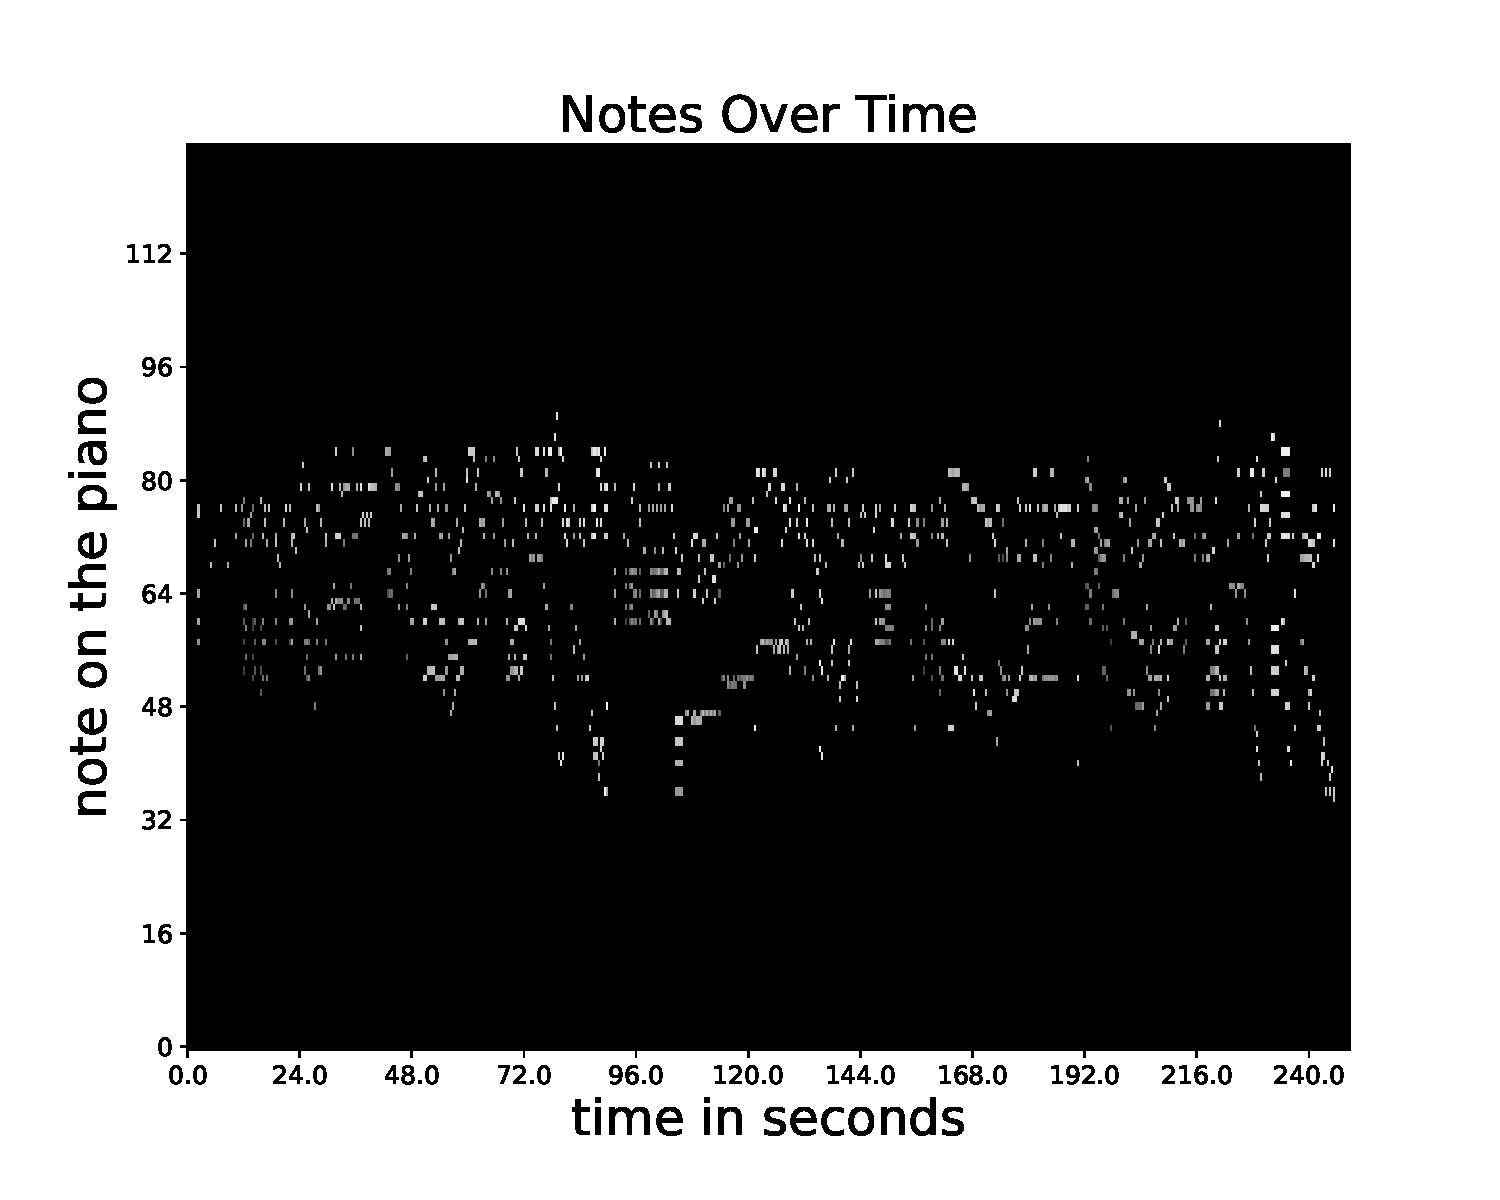
\includegraphics[trim={0 0 0 0},clip,width=0.95\linewidth]{tree_music(original mozart)}
    \centering
    \caption{
        Representation of Mozart Piano Sonata No. 8 in A 
    Minor, K.310, 1st Movement. As with all compositions by Mozart, musical 
    patterns and structure are clearly evident.
    }
\end{figure}

\newpage

\begin{figure}[H]
\centering
\begin{subfigure}
   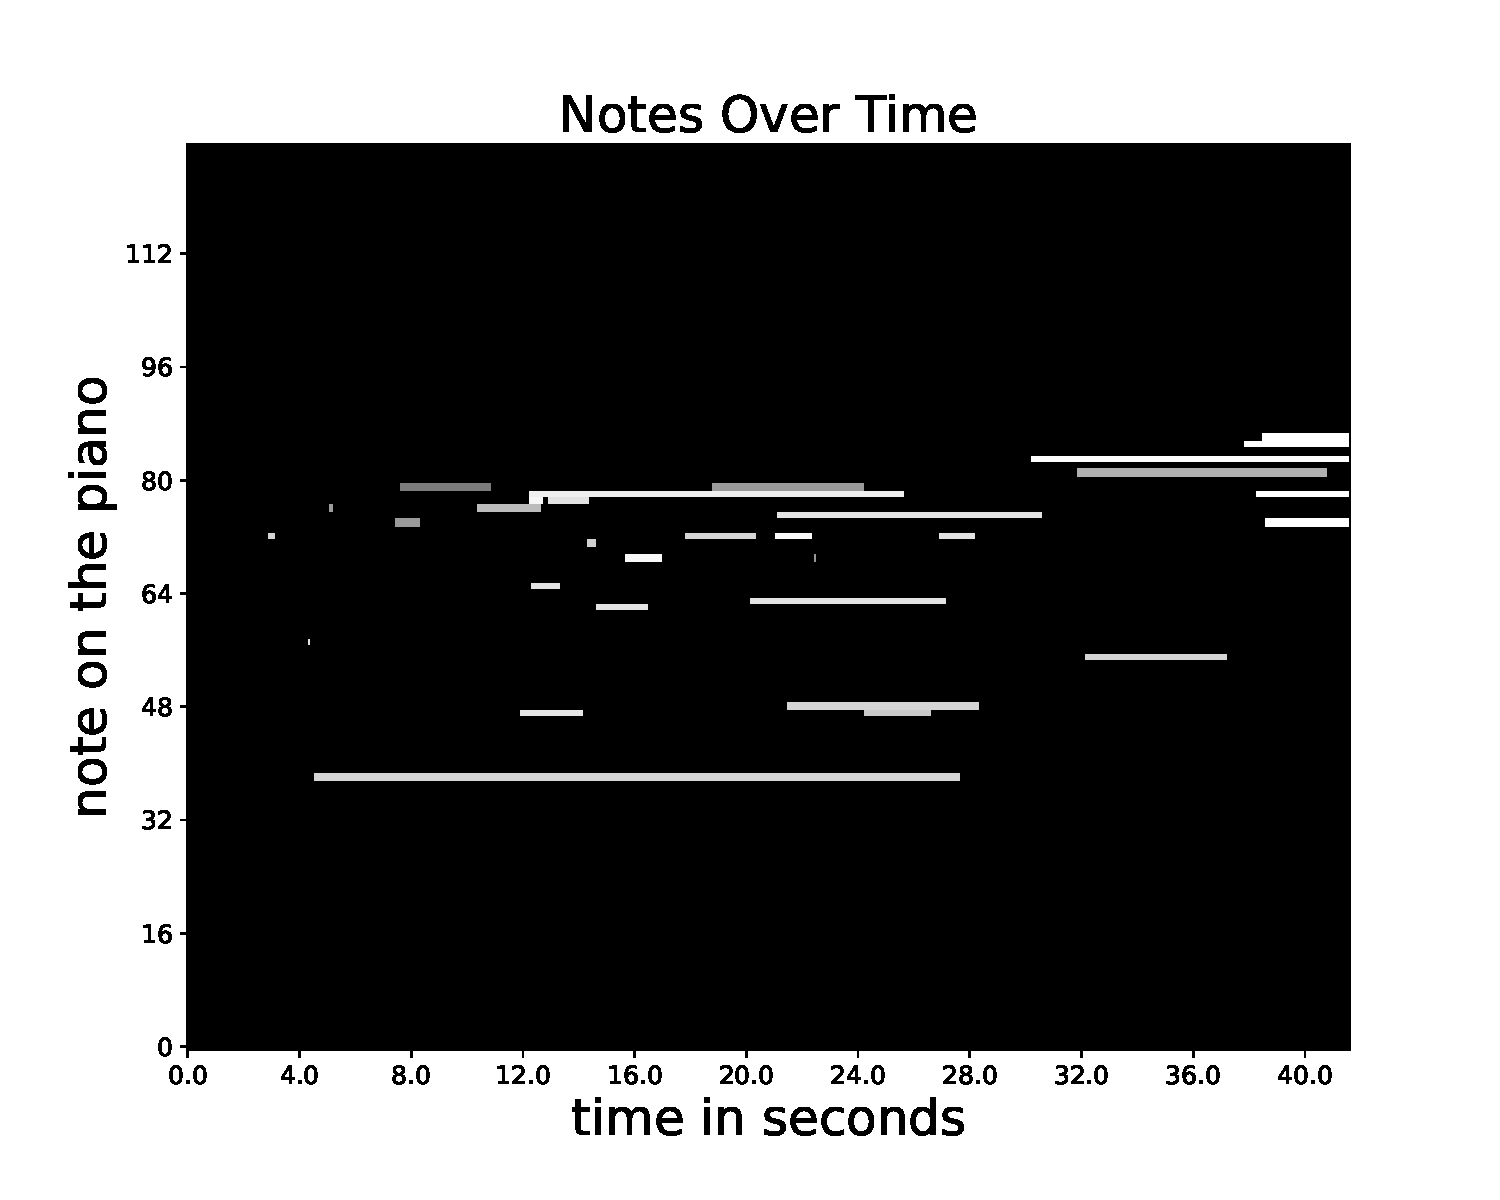
\includegraphics[width=0.95\linewidth]{first_hmm.pdf}

\end{subfigure}

\begin{subfigure}
   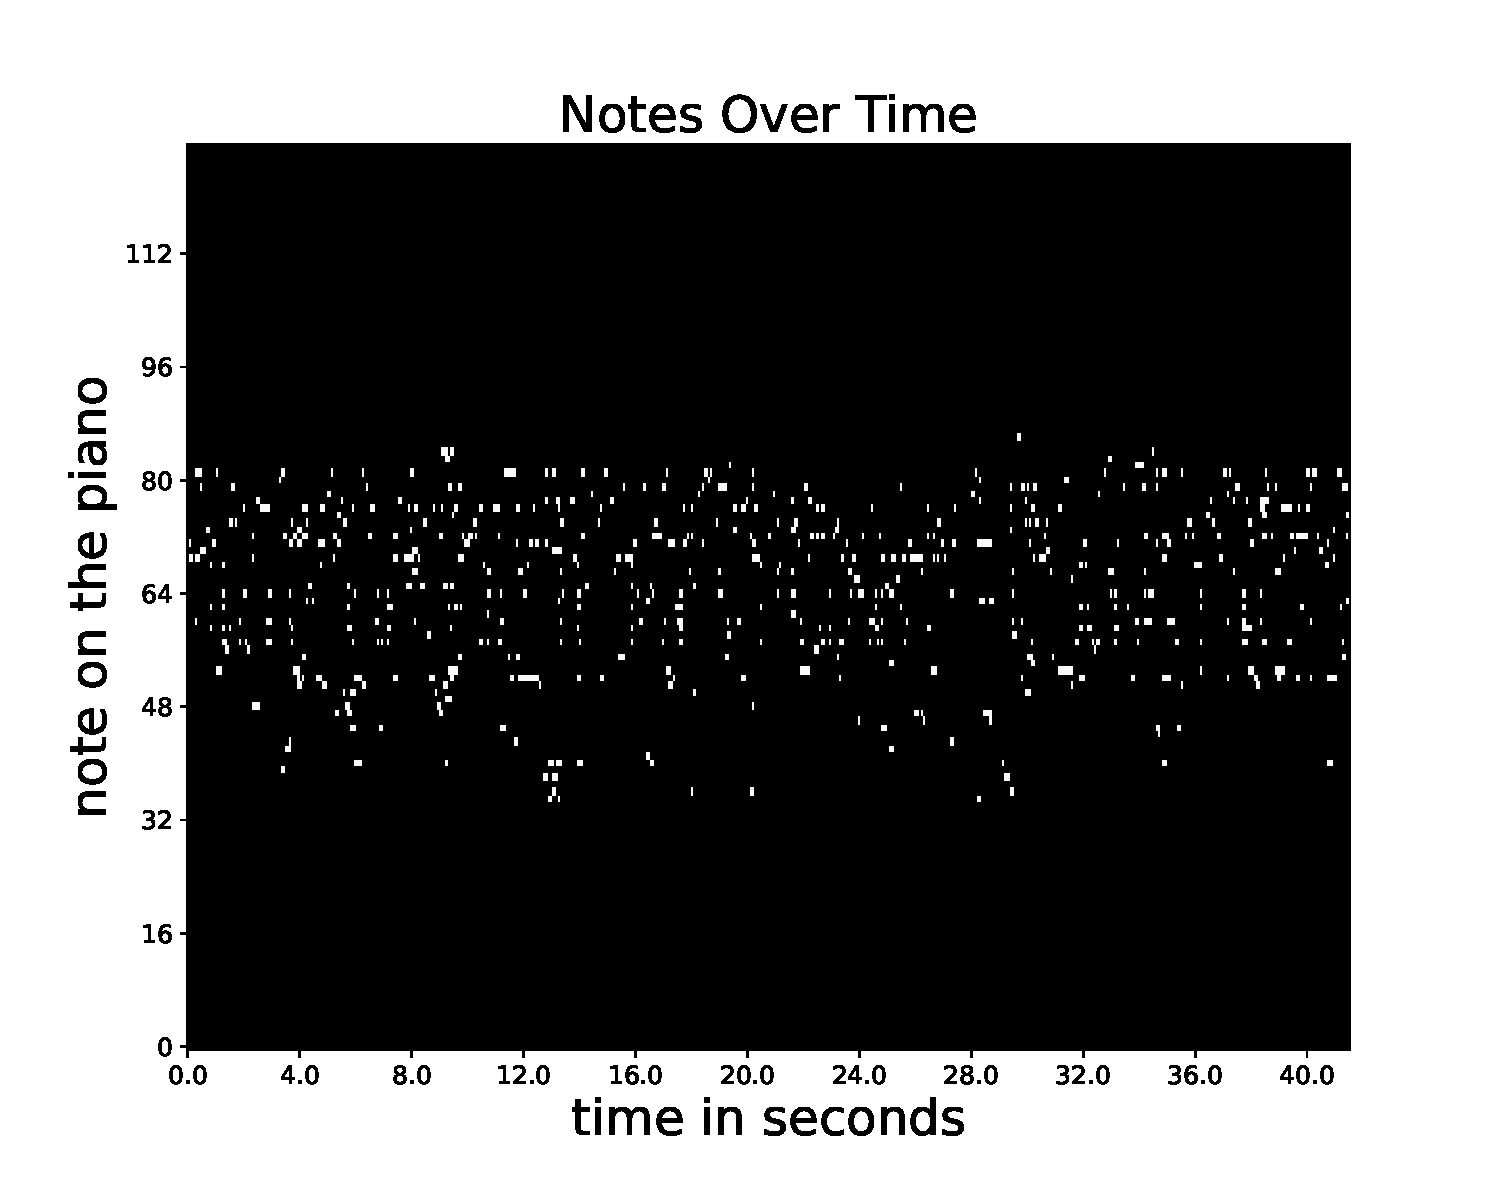
\includegraphics[width=0.95\linewidth]{tree_music(rand_forest attempt).pdf}
\end{subfigure}

\end{figure}

\begin{figure}[H]
\begin{subfigure}
   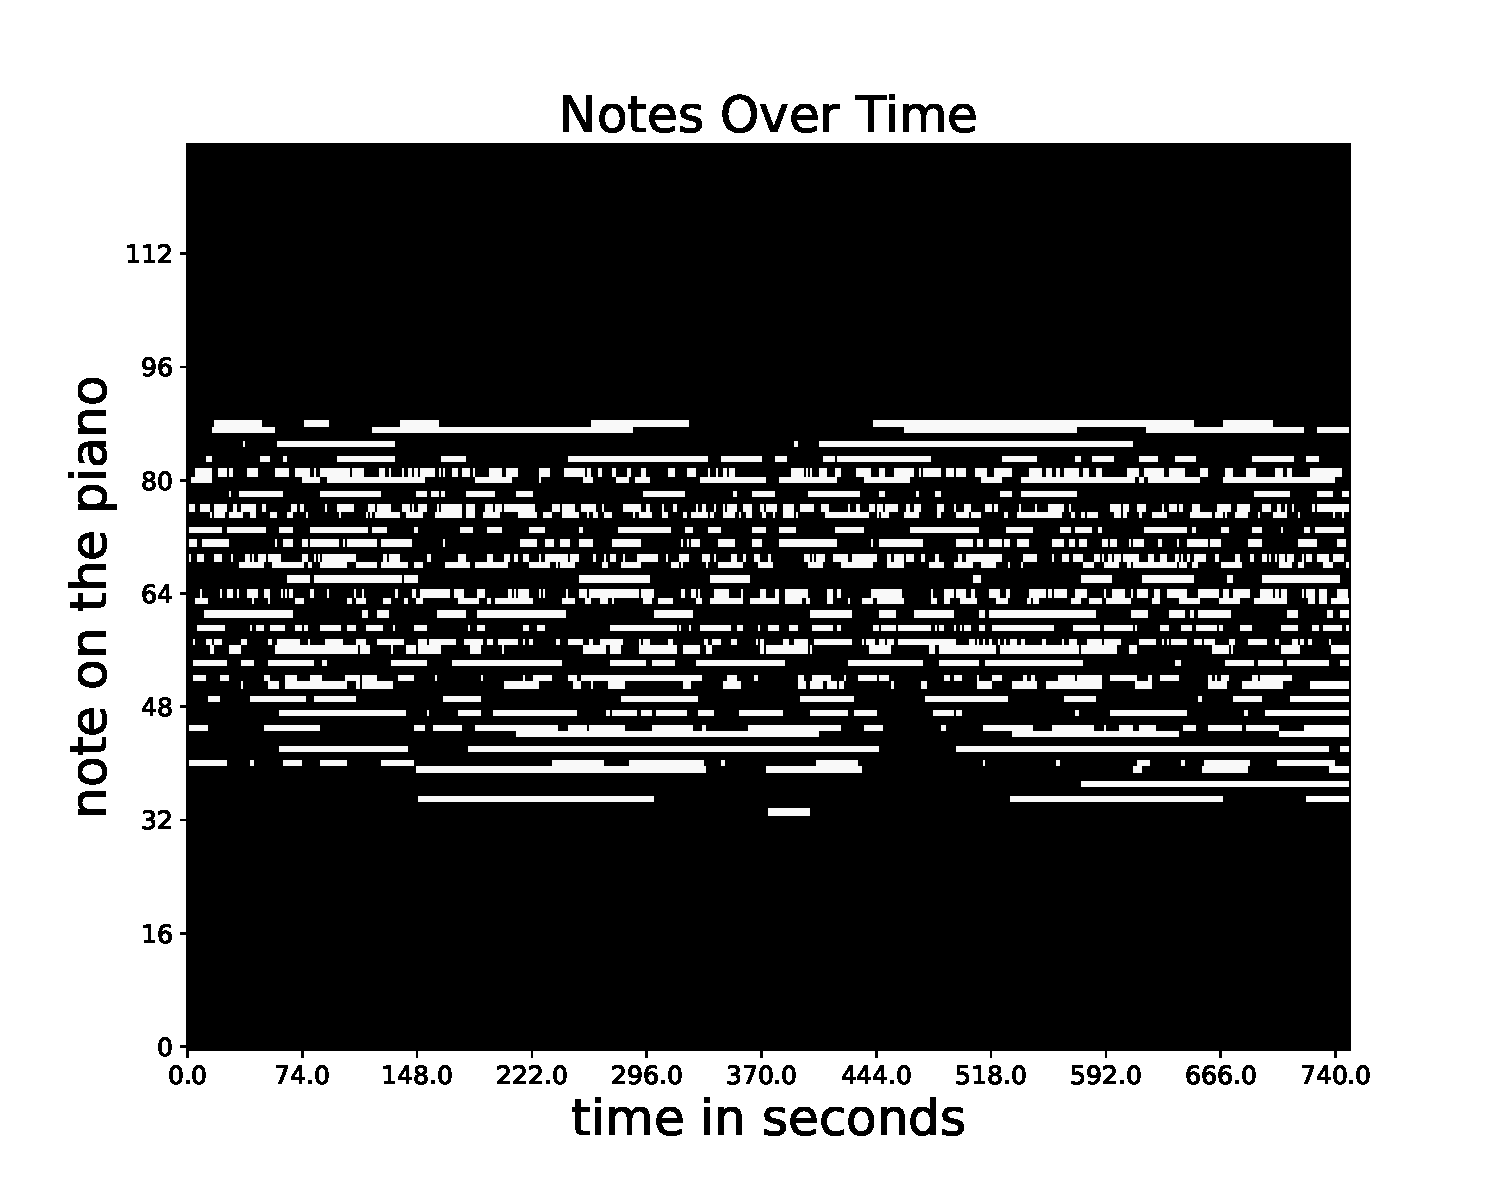
\includegraphics[trim={0 0 0 0},clip,width=1\linewidth]{final_hmm_song.pdf}
   
   \caption{Attempt 1 (top on previous page) clearly had a number of large holes, and it didn't accurately predict how long each note should be pressed. Attempt 2 (bottom on previous page), though not free from error, yielded much better results for both note duration and overall structure, and an attempt at musical patterns is also evident. Attempt 3 (above) has clear elements of structure, though not in the same style as Mozart. The note durations are much more varied than in any of the previous attempts or in Mozart's music.}
\end{subfigure}

\end{figure}

\section{Analysis}
In the end, the program we developed for this project succeeded in generating
music. Our first attempt using a Hidden Markov Model generated music that sounded cluttered, loud, and random. Our second attempt with a Random Forest yielded promising results that were tonal albeit cluttered. Nevertheless, the untrained ear could definitely detect patterns and general ideas developing as the music progressed. Our third attempt far surpassed both previous attempts. This attempt used all of the methods we developed for this project and trained on many pieces by Mozart. The resulting song came out tonal and utilized chords and musical resolutions. That being said, the song sounded more contemporary than Classical Mozart. Though the last song was subjectively the most euphonious, it was far from perfect. There were plenty of notes that sounded clunky or out of place. As a result, the music we generated cannot be mistaken for a piece written by Mozart.

Classical music strove to maintain the rigorous musical structure 
developed during the Baroque Period, but it also sought to make music more 
enjoyable and pleasant to the ear than it was during much of that time. 
While the first goal of Classical music is relatively quantifiable (that is,
musical theory has mathematical properties), the second goal is very difficult to
quantify. While some deep learning algorithms have been successful at replicating Classical music, our limited models found such a complex task too difficult to perform.

\section{Ethical Considerations}
There are a few ethical problems to consider with our project. To begin with, any algorithm like the ones we created for this project should only be trained with music that has either been authorized by the creator or which is public domain. But even then, if a model is trained on music from a certain artist, the new music it generates might infringe on copyright law. This could happen in a few ways. For one, the model might produce music that directly uses musical phrases written by the artist. But even if all of the music is entirely new, its purpose is still to sound as much like the original artist as possible, and a product that is essentially the same as another could be found to infringe on copyright.

Perhaps the biggest ethical concern is that such an algorithm could potentially be used to displace artists. Instead of encouraging creativity, it would stunt creativity in favor of inexpensive production. And if producers are favoring machines to output music, composers would soon find themselves out of a job, and musical culture would languish without the funding it needs to progress.

\section{Conclusion}
In conclusion, we made progress in the area of non-neural music generation by using \textit{HMM}s and Random Forests to generate unique musical content. However, we were not able replicate Mozart's style of composition in a way we found satisfactory, which was our primary objective. Though our final results are quite promising, we believe that non-neural algorithms have a long way to go if they will ever be able to replicate the complexities of music and human emotion.


\printbibliography
\end{document}